\documentclass[11.5pt,twoside]{book}
\usepackage{graphicx}
\usepackage{fontbook}
\usepackage[colorlinks=false, pdfborder={0 0 0}, pdftitle={Open Font Format Specification for Scripts of India},
  pdfauthor={Santhosh Thottingal}, pdfsubject={Open Font Format Specification}, pdfkeywords={Font, indic, open , scripts , india}]{hyperref}

%---------------------------------------------------

\begin{document}
%% Set mininum characters on left and right for hyphenation
\lefthyphenmin=3
\righthyphenmin=5
%\normalsize=11.5pt

%-----------------------------Cover Page----------------------------------------

%\includepdf{cover}

%------------------------------Title Page --------------------------------------
\begin{center}

\vspace*{2 in}

\HRule \\[0.4cm]
{\huge \bfseries Open Font Format Specification for Scripts of India}
\\
{\small \bfseries Elaborate, Illustrated font development guideline document
for scripts of India by font designers, developers, language experts.}
\\
\HRule \\[0.4cm]

\emph{Author}\\
Santhosh \textsc{Thottingal}


\vfill

{\large \today}

\end{center}
\thispagestyle{empty}
%%%%%%%%%%%%%%%%%%%%%%%%%%%%%%%%%%%%%%%%%%%%%%%%%%%%%%%%%%%%%%%%%%%%%%%%
% -------------------------Dedication----------------------------------%
%%%%%%%%%%%%%%%%%%%%%%%%%%%%%%%%%%%%%%%%%%%%%%%%%%%%%%%%%%%%%%%%%%%%%%%%
\frontmatter
~
\vfill
\begin{center}Dedicated to all font designers\end{center}
\vfill
~
\thispagestyle{empty}
\newpage

%%%%%%%%%%%%%%%%%%%%%%%%%%%%%%%%%%%%%%%%%%%%%%%%%%%%%%%%%%%%%%%%%%%%%%%%
% Auto-generated table of contents, list of figures and list of tables %
%%%%%%%%%%%%%%%%%%%%%%%%%%%%%%%%%%%%%%%%%%%%%%%%%%%%%%%%%%%%%%%%%%%%%%%%
\tableofcontents
\thispagestyle{empty}
%\listoffigures
%\listoftables

\mainmatter
%%%%%%%%%%%%
% Chapters %
%%%%%%%%%%%%
\chapter{Introduction}

%\begin{chapquote}{Author's name, \textit{Source of this quote}}
%``This is a quote and I don't know who said this.''
%\end{chapquote}

\secstar{Need for document}

In the present era, if we simply compare the availability of Latin and Indian fonts we can easily observe a large difference. Only a handful of fonts are available for Indian languages compared to the thousands of fonts in a wide  variety of styles that are available for Latin script.

\secstar{Objectives of document}

\secstar{Target Audience for this document}

\secstar{Scope}
\begin{itemize}
\item This document covers only languages and scripts recognized in India.
\item This document covers all complex OFF features required for Indian scripts.
\item This document is based on the current expertise of community members working in this area.
\item This document is from the typography perspective for each script and many not be linguistically correct.
\item This document does not cover design or calligraphy style aspects but covers only technical aspects.
\item This document is based on Unicode 6.2 and ISO/IEC 14496-22:2009 (Second Edition) "Open Font Format" standard.
\item This document is not a tutorial on font design or development and does not teach typography.
\end{itemize}

\secstar{How to use this document}

Elaborate, Illustrated font design guideline document for Indic fonts by font designers, developers, language experts.
- designer freedom to adapt

\secstar{Notes on Collaboration}

\chapter{General Concepts}

\section{Script}
At least one set of defined base elements or symbols,  is a requirement for all
writing systems. these symbols are individually termed as characters and
collectively called a script. simply  the set of the symbols required to
represent a writing system is called a script. a script may in turn be used to
represent more than one languages. Latin, Devanagari and Arabic are examples of
scripts. English, French, German, and Latin are all languages written using the
Latin script.

\section{Complex script }
\begin{wrapfigure}{r}{0.4\textwidth}
\begin{center}
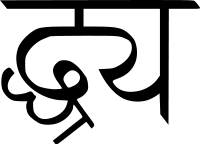
\includegraphics[width=0.2\textwidth,height=0.2\textwidth,keepaspectratio]{
JanaSanskritSans_ddhrya.png}

{\tiny The Devanagari ddhrya-ligature, as displayed in the JanaSanskritSans
font.}
\end{center}
\end{wrapfigure}


Complex script is a writing system in which the shape or positioning of a
character
depends on its relation to other characters.

What makes it complex?
* Bi-directional: text is written right-to-left (For example: Arabic, Hebrew)
and left-to-right (For example: Devanagari)

* Context sensitive shaping and ligatures: Character may change shape depending
upon position.

* Ordering:
In Gujarati, Ki is where 'i' is place before 'K'.

//FIXME
What is a complex script? What makes it complex, some examples, screenshots
2-3 paragraph + images
How it differs from simple scripts like Latin Character

\section{Glyph }

A glyph is an element of writing. It can be a single character or a group of
characters.
Visually, if you see one or more characters form a single visual unit, it is
called a glyph.

In typography, it is "the specific shape, design, or representation of a
character".
\footnote{Ilene Strizver. "Confusing (and Frequently Misused) Type Terminology,
Part 1". fonts.com. Monotype Imaging.}

It is a particular graphical representation, in a particular typeface, of an
element of written language, which could be a grapheme, or part of a grapheme,
or sometimes several graphemes in combination.

To illustrate this concept, a set glyphs inside a Latin font (Fig.
\ref{Robotoglyph}) and a Malayalam font  (Fig. \ref{Meeraglyph}) as seen in
fontforge is given below.

\begin{figure}[h]
    \centering
    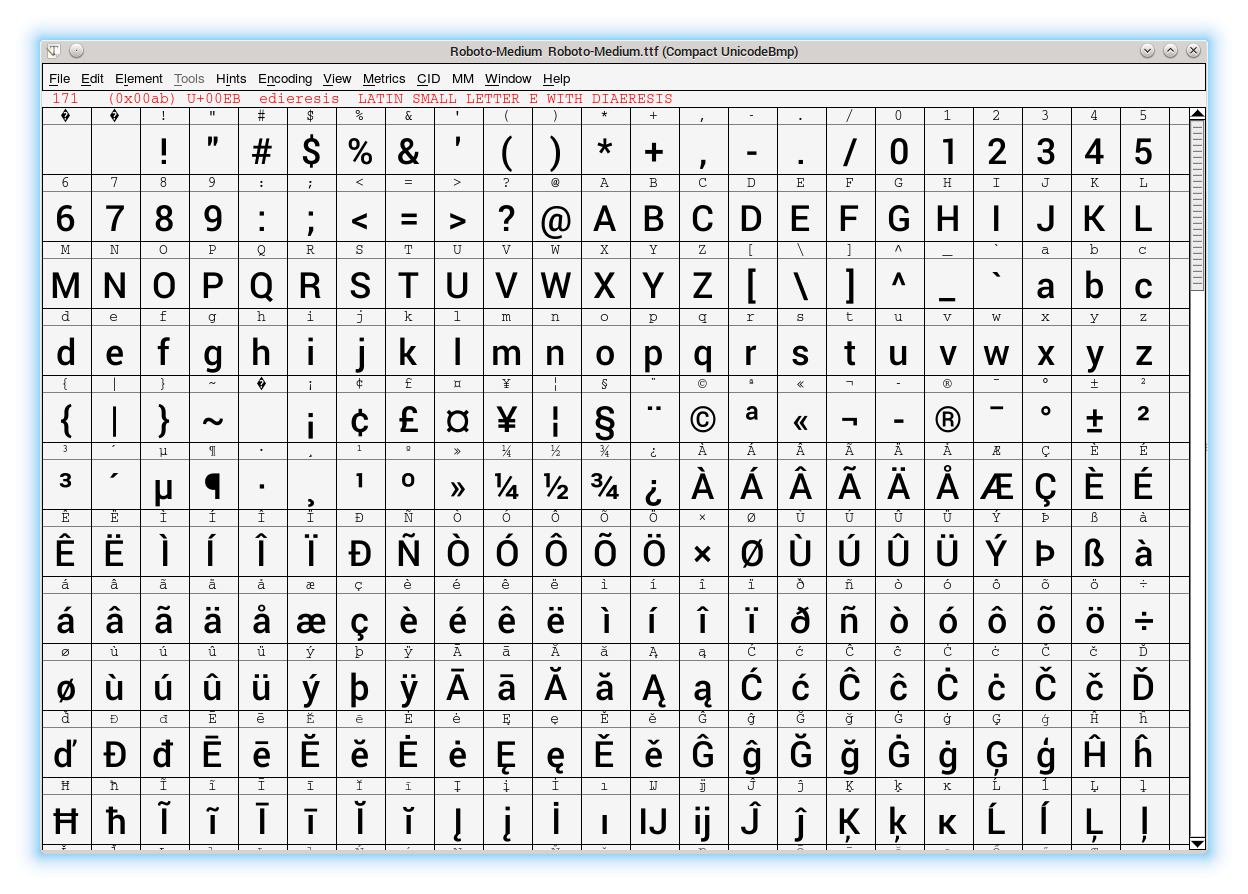
\includegraphics[width=0.8\textwidth]{glyph-fontforge-roboto.png}
    \caption{Glyphs inside Roboto font}
	\label{Robotoglyph}
\end{figure}

\begin{figure}[h]
    \centering
    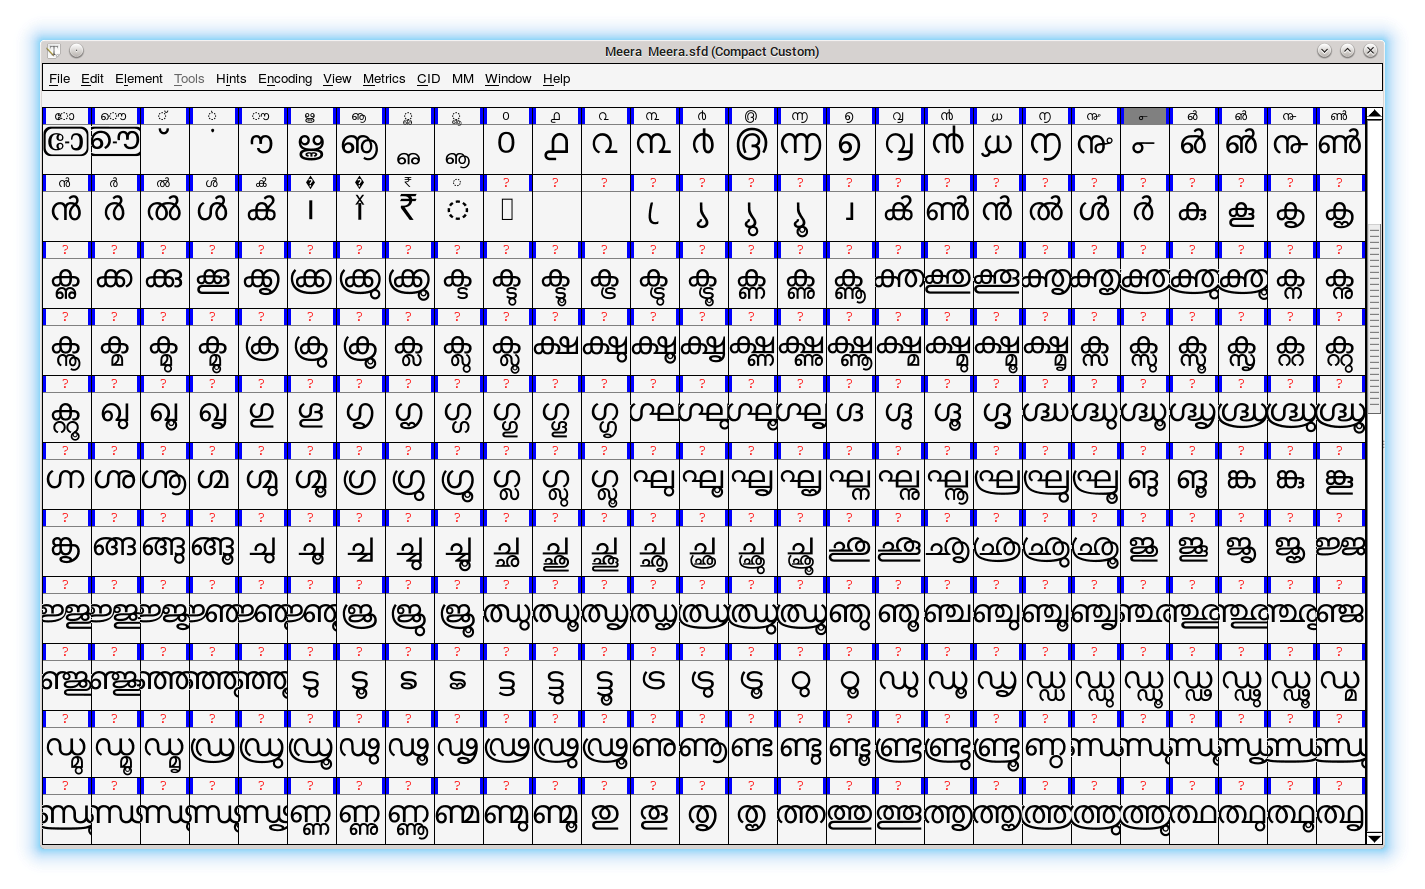
\includegraphics[width=0.8\textwidth]{glyph-fontforge-meera.png}
    \caption{Glyphs inside Meera font}
	\label{Meeraglyph}
\end{figure}

\begin{figure}[h]
    \centering
    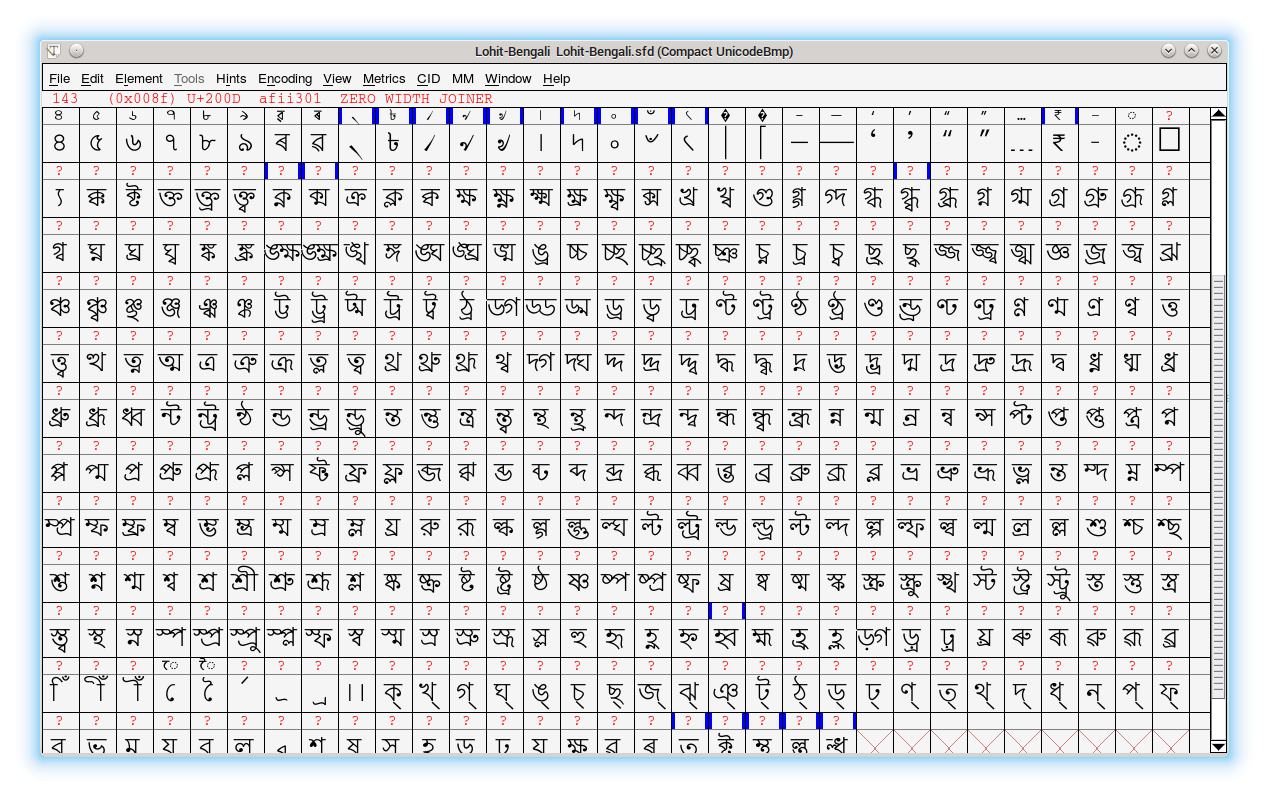
\includegraphics[width=0.8\textwidth]{glyph-fontforge-lohit-bengali.png}
    \caption{Glyphs inside Lohit Bengali font}
\end{figure}

\section{Ligatures }

In writing and typography, a ligature occurs where two or more graphemes or
letters are joined as a single glyph. Ligatures usually replace consecutive
characters sharing common components and are part of a more general class of
glyphs called "contextual forms", where the specific shape of a letter depends
on context such as surrounding letters or proximity to the end of a line.
\footnote{\url{https://en.wikipedia.org/wiki/Typographic_ligature}}

By way of example, the common ampersand '\&' represents the Latin conjunctive
word et, for which the English equivalent is the word "and". The ampersand's
symbol is a ligature, joining the old handwritten Latin letters e and t of the
word et, so that the word is represented as a single glyph.

The Brahmic abugidas make frequent use of ligatures in consonant clusters. The
number of ligatures employed may be language-dependent; thus many more ligatures
are conventionally used in Devanagari when writing Sanskrit than when writing
Hindi. Having 37 consonants in total, the total number of ligatures that can be
formed in Devanagari using only two letters is 1369, though few fonts are able
to render all of them.

\begin{figure}[h]
   \centering
   {\hindi\textexample द्ध्र्य }
   \caption{The Devanagari ddhrya-ligature {\hindi (द् + ध् + र् + य = द्ध्र्य)
} }
\end{figure}

\begin{figure}[h]
   \centering
   {\malayalam\textexample  ക്തു}
   \caption{The Malayalam kthu-ligature {\malayalam (ക + ് + ത + ു ) } }
\end{figure}

\begin{figure}[h]
  \centering
  {\gujarati\textexample સ +  ં = સં}
  \caption{The Gujarati 's' formed from SA and ANUSVARA}
\end{figure}

\section{Cluster/Syllable }

\section{Akhand }

\section{Ra Forms }
//FIXME
Explain Reph
Explain Rakar

\subsection*{Matra}
//FIXME
Explain prebase, postbase matra with examples and images

\section{Split Matra }

\section{Reordering }

\section{Zero Width Joiner }

\section{Zero Width Non Joiner }

\section{Stacking }


\chapter{Open font format}

\section{Introduction}

\section{GPOS}

\section{GSUB}

\section{GDEF}

\section{Shaping Engine}

[Some conent from http://behdad.org/text/ can be used ]
\section{Shape Glyph sequence}

\section{Position Glyph sequence}

\section{Reference fonts}

To illustrate the concepts in this document, we will be using a set of reference fonts for each script, some times more than one per script. 
List of fonts table

\section{Reference Rendering Engine}

We are using Harfbuzz as  a reference rendering engine. Examples given are working perfectly with Harfbuzz but any rendering engine conforms to the Open font specification will give same result.


\chapter{Bengali}
\section{Introduction}

\section{Reference fonts}

\subsection{Lohit Bengali}

Lohit Bengali is one of the popular fonts for Bengali.

\subsection{History}
In 2004, Red Hat released five fonts for the Indian language under GPL 2.
The fonts were originally developed by Modular Infotech
\footnote{Modular Infotech \url{http://www.modular-infotech.com/}}.
In 2011, Red Hat relicensed fonts under SIL OFL 1.1 license
\footnote{License change announcement of Lohit fonts
\url{https://www.redhat.com/archives/lohit-devel-list/2011-September/msg00000.html}}.
The fonts named Lohit which means Red in Sanskrit. Currently, the font family
supports 21 Indian languages: Assamese, Bengali, Devanagari (Hindi, Kashmiri,
Konkani, Maithili, Marathi, Nepali, Sindhi, Santali, Bodo, Dogri), Gujarati,
Kannada, Malayalam, Manipuri, Odiya, Punjabi, Tamil, and Telugu.

Now, Fedora Project and its contributors took the responsibility to consolidate
the further efforts and improvements of the Lohit fonts.

Homepage: {\url{https://fedorahosted.org/lohit/}}

\chapter{Devanagari}
\section{Introduction}

Devanagari is an abugida alphabet for India and Nepal. Devanagari is used to
write Standard Hindi, Marathi, Nepali along with Awadhi, Bodo, Bhojpuri,
Gujari, Pahari, (Garhwali and Kumaoni), Konkani, Magahi, Maithili, Marwari,
Bhili, Newar, Santhali, Tharu, and sometimes Sindhi, Dogri, Sherpa, Kashmiri
and Punjabi. It was formerly used to write Gujarati. Because it is the
standardized script for the Hindi language, Devanagari is one of the most used
and adopted writing systems in the world.

\section{Reference fonts}

\subsection{Lohit Devanagari}
Lohit Devanagari font is consider as most popular Devanagari font in India.
Gargi, Chandas, Kalimati, Samanata, Nakula are other popular free and
opensource fonts available.

We will take Lohit Devanagari as reference font.

\subsection{History}
In 2004, Red Hat released five Indian language fonts as open source licensed
under the GPL. In 2011, Red Hat relicensed fonts under SIL OFL 1.1 license.
The fonts named Lohit which means Red in Sanskrit. Currently, the font family
supports 21 Indian languages: Assamese, Bengali, Devanagari (Hindi, Kashmiri,
Konkani, Maithili, Marathi, Nepali, Sindhi, Santhali, Bodo, Dogri), Gujarati,
Kannada, Malayalam, Manipuri, Odiya, Punjabi, Tamil, and Telugu.

Now, Fedora Project and its contributors took the responsibility to consolidate
the further efforts and improvements of the Lohit fonts.

Homepage: {\url{https://fedorahosted.org/lohit/}}

\chapter{Gujarati}
\section{Introduction}

Gujarati script is an abugida like many other Indic scripts rather than
alphabet. It is used for languages like Gujarati and Kutchi. Gujarati script is
variant of Devanagari script differentiated by the loss of the characteristic
horizontal line running above the letters and by a small number of
modifications in the remaining characters.

The modern Gujarati alphabet has 13 vowel letters, 36 consonant letters, 12
vowel extensions and few other symbols.

\section{Reference fonts}

We will use Lohit Gujarati as reference font as of now. Other popular Unicode
Gujarati fonts are: Shruti (non free, Microsoft), Rekha, Aakar and Kalapi. Arial
MS Unicode is often used as default Gujarati font and Gujarati MT is popular
default Gujarati font in Mac OS X.

\subsection{Lohit Gujarati}
// FIXME: Short introduction, designers, maintainers, usage info, popularity of
the font.

Lohit Gujarati font is consider as one of the most popular OpenSource Gujarati
font.

\subsection{History}
In 2004, Red Hat released five Indian language fonts as open source licensed
under the GPL. In 2011, Red Hat relicensed fonts under SIL OFL 1.1 license.
The fonts named Lohit which means Red in Sanskrit. Currently, the font family
supports 21 Indian languages: Assamese, Bengali, Devanagari (Hindi, Kashmiri,
Konkani, Maithili, Marathi, Nepali, Sindhi, Santali, Bodo, Dogri), Gujarati,
Kannada, Malayalam, Manipuri, Odiya, Punjabi, Tamil, and Telugu.

Now, Fedora Project and its contributors took the responsibility to consolidate
the further efforts and improvements of the Lohit fonts.

Homepage: {\url{https://fedorahosted.org/lohit/}}


\chapter{Kannada}

\chapter{Malayalam}
\secstar{Introduction}

Like many other Indic scripts, it is an abugida, or a writing system
that is partially “alphabetic” and partially syllable-based. The
modern Malayalam alphabet has 13 vowel letters, 36 consonant letters,
and a few other symbols. The Malayalam script is a Vattezhuttu script,
which had been extended with Grantha script symbols to represent
Indo-Aryan loanwords. The script is also used to write several
minority languages such as Paniya, Betta Kurumba, and Ravula. The
Malayalam language itself was historically written in several
different scripts.

As is the case for many other Brahmi-derived scripts in the Unicode
Standard, Malayalam uses a virama character to form consonant
conjuncts. The virama sign itself is known as candrakala(ചന്ദ്രക്കല) in
Malayalam.

When the candrakala sign is visibly shown in Malayalam, it usually
indicates the suppression of the inherent vowel, but it sometimes
indicates instead a reduced schwa sound, often called “half-u” or
samvruthokaram. In the later case, there can also be a -u vowel sign,
and the base character can be a vowel letter. In all cases, the
candrakala sign is represented by the character U+0D4D malayalam sign
virama, which follows any vowel sign that may be present and precedes
any anusvara that may be present.

FIXME samvruthokaram needs more explanation, refer
{\url{http://thottingal.in/documents/Malayalam_Unicode_Report_of_Workshop_Kerala_University.pdf}}
and {\url{http://smc.org.in/doc/rachana-malayalam-collation.pdf}}

\secstar{Orthography variation}

Malayalam has two orthography variations, both actively
used. Generally they are known as Old orthography and Modern
orthography. Old orthography is also known as traditional
orthography. Modern orthography is also known as reformed orthography.

Old orthography is generally identified by large number of ligature
glyphs, often formed by more than one consonants or vowel
combination. For example, in old orthography, consonant {\meera ക} +
vowel { \meera ൂ} will form കൂ as a single ligature. similarly a
conjunct {\meera ക + ് + ത} will form {\meera ക്ത} as a single
ligature. Font developers of traditional stye fonts design and draw
this large set of glyphs. For a reference font Meera, the number of
glyphs is approximately over a thousad.

In the 1970s and 1980s, Malayalam underwent orthographic reform due to
printing difficulties. The treatment of the combining vowel signs u
and uu was simplified at this time. These vowel signs had previously
been represented using special cluster graphemes where the vowel signs
were fused beneath their consonants, but in the reformed orthography
they are represented by spacing characters following their consonants.

// FIXME: insert image here to illustrate both orthography
variation. Refer chapter 9 of Unicode standard page 307 for a sample
image

\secstar{Reference fonts}

Since we need to illustrate both orthographies we will be using 2
fonts. For old orthography, we will use Meera font and for modern
orthography we will use Lohit Malayalam.

\subsection {Meera Font}
{\meera മീര മാതൃക }
// FIXME: Short introduction, designers, maintainers, usage infor,
popularity of the font

\subsection {Lohit Malayalam Font}
// FIXME: Short introduction, designers, maintainers, usage infor,
popularity of the font

\chapter{Odiya}

\chapter{Panjabi}

\chapter{Tamil}

\chapter{Telugu}

\chapter{Glossary}

\chapter{References}

State of Text Rendering By Behdad Esfahbod <behdad behdad com>   http://behdad.org/text/ 


\chapter{Appendices}

[Editor notes]


\end{document}
